\section{Impressum}
Das Projektteam besteht aus folgenden Schülern:\\

\begin{table}
    \begin{center}
    \begin{tabular}{|p{0.2\textwidth}|p{0.55\textwidth}|p{0.25\textwidth}|}
      \hline
      \textbf{Name} & \textbf{Aufgabenstellung} & \textbf{Bild} \\
      \hline
      Paul Hartmann & Paul übernahm die Projektleitung und war für die Kommunikation mit dem Partnerunternehmen zuständig. Er recherchierte zu Varianten zur Lagerung von Fahrrädern und führte die Nutzwertanalyse und Umfrage aus. Paul entwickelte die Mobile-App. & \begin{minipage}{.3\textwidth} 
\includegraphics{images/paulhartmann.jpg} \end{minipage}\\
      \hline
      Joshua Lung & Joshua recherchierte zu Varianten zur Lagerung von Fahrrädern, führte die Nutzwertanalyse aus, erstellte Fragen der Umfrage und konzeptionierte das Rondell-Modell. Er baute den Prototyp des Turmes und übernahm die Softwareentwicklung der Steuerung. & \begin{minipage}{.3\textwidth}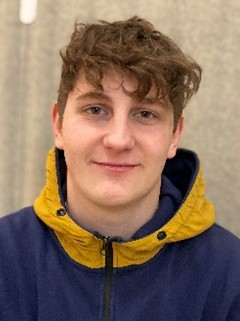
\includegraphics{images/joshualung.jpg} \end{minipage}\\
      \hline
      Lukas Madlener & Lukas erstellte Skizzen für verschiedene automatisierte Arten zur Lagerung von Fahrrädern und konzeptionierte das Hochregallager. Er testete NFC-Technologien mit einer Mobile-App. & \begin{minipage}{.3\textwidth}
\includegraphics{images/lukasmadlener.jpg} \end{minipage}\\
    \end{tabular}
    \caption{Projektteam}
    \label{tab:projektteam}
    \end{center}
\end{table}